\documentclass[aspectratio=169]{beamer}
\beamertemplatenavigationsymbolsempty

% Internal Beamer navigation combined with video.  Beamer writes \hyperlink
% targets as PDF link annotations, which beampptx turns into PowerPoint slide
% jumps.  This file exercises the cases that interact badly with other slide
% content: overlays (the target must resolve to the right expanded slide) and
% videos (a link rectangle drawn on top of a movie can swallow the click that
% would otherwise start playback).
\usepackage{multimedia}

\title{Beamer with Internal Navigation}
\author{Author Name}
\date{\today}

\begin{document}

\begin{frame}
    \titlepage
\end{frame}

\begin{frame}[label=menu]{Menu}
    Each button below jumps to a labelled frame later in the deck.
    \begin{center}
        \hyperlink{overlays}{\beamergotobutton{Overlays}}
        \hspace{1em}
        \hyperlink{video}{\beamergotobutton{Video}}
        \hspace{1em}
        \hyperlink{covered}{\beamergotobutton{Link over video}}
    \end{center}

    A link may also target a specific overlay rather than the first one:
    \begin{center}
        \hyperlink{overlays<3>}{\beamergotobutton{Overlays, third state}}
    \end{center}
\end{frame}

\begin{frame}[label=overlays]{Overlays}
    Beamer expands this frame into three slides, so the two buttons on the
    menu must land on different PowerPoint slides.
    \pause
    Second state.
    \pause
    Third state --- this is what \texttt{overlays<3>} should reach.
    \begin{center}
        \hyperlink{menu}{\beamerreturnbutton{Back}}
    \end{center}
\end{frame}

\begin{frame}[label=video]{Video Beside a Link}
    The button sits clear of the movie, so both should stay clickable.
    \begin{center}
        \movie[width=0.5\linewidth,height=0.28\linewidth,poster,showcontrols]
              {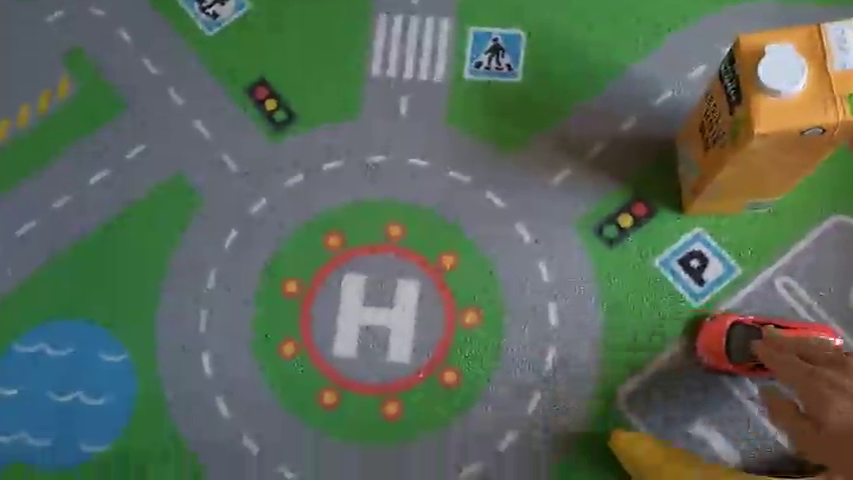
\includegraphics[width=0.5\linewidth,height=0.28\linewidth]{video_snap.png}}
              {video.mp4}
    \end{center}
    \begin{center}
        \hyperlink{covered}{\beamergotobutton{Next test}}
    \end{center}
\end{frame}

\begin{frame}[label=covered]{Link Covering a Video}
    Here the whole movie is wrapped in \texttt{\textbackslash hyperlink}, so the
    link rectangle covers the video exactly.  In the generated PPTX the click
    action and the media shape compete for the same area.
    \begin{center}
        \hyperlink{overlays}{%
            \movie[width=0.5\linewidth,height=0.28\linewidth,poster,showcontrols]
                  {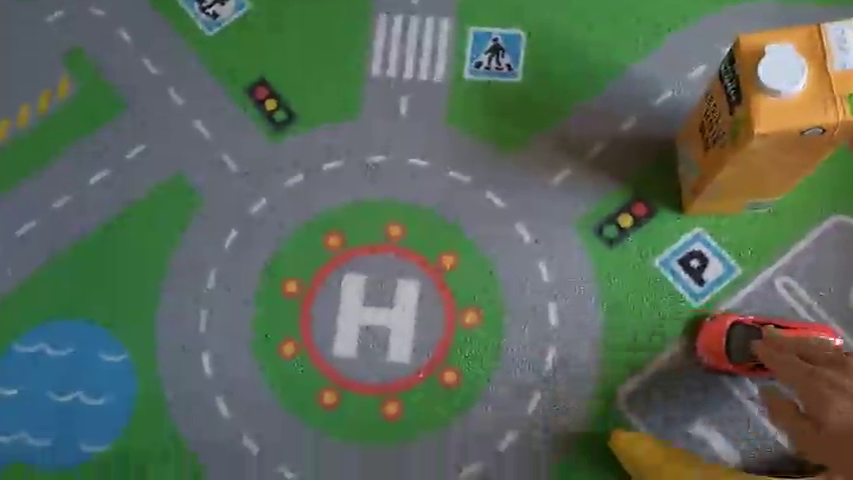
\includegraphics[width=0.5\linewidth,height=0.28\linewidth]{video_snap.png}}
                  {video.mp4}%
        }
    \end{center}
    \begin{center}
        \hyperlink{menu}{\beamerreturnbutton{Back to menu}}
    \end{center}
\end{frame}

\end{document}
